%!TEX root = ../tudkom_students__201804_v1.4.tex
\chapter{Evaluation}
\label{ch:evaluation}
%This chapter should describe how the evaluation of the implemented mechanism was done.
%1. Which evaluation method is used and why? Simulations, prototype?
%2. What is the goal of the evaluation? Comparison? Proof of concept?
%3. Wich metrics are used for characterizing the performance, costs, fairness, and efficiency of the system?
%4. What are the parameter settings used in the evaluation and why? If possible always justify why a certain threshold has been chose for a particular parameter.
%5. What is the outcome of the evaluation?
% 5-10 pages

\section{Ziele}
\label{ch:aimEval}
Mit dem Wearable werden einige Tests mit Blick auf die in der Einleitung \ref{ch:aims} aufgestellten Ziele durchgeführt.
Die Austauschbarkeit der Protokolle und Komponenten wird durch die Implementierung erreicht.
Insbesondere die Trennung des Codes von Endgerät, MCU, IMU und dem Protokoll zwischen MCU und IMU tragen dazu bei.
Ob die Größe und das Gewicht ausreichend gering sind, ist vom Anwendungsfall abhängig.
Bei dem Wearable sind sie stark von der Knopfzelle geprägt.
Es wurde die etwa 2.36 cm\textsuperscript{3} große CR2450 statt der etwa 1.01 cm\textsuperscript{3} großen CR2032 gewählt um die 2.7-fache Kapazität zu erhalten.
Um die Entscheidung zu ändern, muss nur das Platinenlayout überarbeitet werden, während das Schaltbild und der Code übernommen werden können.
Ob die Kapazität der Knopfzellen überhaupt anwendungstauglich ist, soll in den Tests zur Stromaufnahme ermittelt werden.
Dafür sollen verschiedene Parameter geändert, der Einfluss auf die Stromaufnahme gemessen und die Auswirkungen auf die Datenübertragung evaluiert werden.
Bei der Datenübertragung wird geprüft, inwieweit die empfangene Datenrate von der eingestellten Sensordatenrate abweicht.\\
Es wird die Stromaufnahme verglichen in den Szenarien Prototyp mit LSM6DSL IMU vs Wearable und LSM6DSL IMU vs BMI160 IMU auf dem Prototypen.
Der Prototyp besteht aus dem nRF52 DK und dem STEVAL-MKI178V2 bzw. BMI160 Shuttle Board.
Die Auswirkungen auf die Stromaufnahme und der Datenübertragung werden auf dem Wearable bei einer Änderung der Größe des TX-Buffers, der MTU-Größe, des Connection Intervals, der SPI-Frequenz und der Sensordatenrate erfasst.
Um den Einfluss des Algorithmus zu erfassen, werden die Test mit der variablen Größe des TX-Buffers auch ohne aktiven Algorithmus getestet.
Dafür wird dem Algorithmus eine Größe des TX-Buffers von 0xFFFFu in \texttt{main.c} in der Zeile \texttt{err\_code = my\_service\_init(\allowbreak{}\&m\_myservice, TX\_QUEUE\_SIZE);} übergeben.

\section{Methoden}
Zur Messung der Datenrate wird auf dem Smartphone angezeigt, wie viele Datenpakete in einer Sekunde ankommen.
Um die Abweichung zur Einstellung zu vergleichen wird die Datenrate pro Sekunde über einen Zeitraum aufgenommen und die Formel \ref{eq:standardabweichung} für die Standardabweichung mit dem unverzerrten Schätzer angewandt.
\begin{equation}
  \label{eq:standardabweichung}
	s = \sqrt{\cfrac{1}{n-1}\sum_{i=1}^{n} (x_{i}-\overline{x})^{2}}\text{, mit $n$ = Anzahl der Werte und $\overline{x}$ = eingestellte Sensordatenrate}
\end{equation}
Die Standardabweichung wird wiederum auf einem Graphen auf dem Smartphone aufgezeichnet, sobald Daten von mindestens 30 Sekunden vorliegen.\\
Um die Stromaufnahme zu messen, wird das ohmsche Gesetz $I = \cfrac{U}{R}$ benötigt.
Wird ein Widerstand in Reihe mit der Spannungsversorgung des Wearables geschaltet, ist ein Spannungsabfall über dem Widerstand zu messen.
Da man den Wert des Widerstandes kennt und den Spannungsabfall mit einem Oszilloskop messen kann, lässt sich mit der Formel der Strom berechnen.
In dem Handbuch des nRF52 DK wird vorgeschlagen, einen 10 Ohm Widerstand zu nehmen. \cite{site_nrf52dk}\\
Bei dem Versuch, damit den Strom während des Schlafmodus zu messen, wird ein Spannungsabfall im Bereich von wenigen nV gemessen.
Durch Störeinflüsse der Umwelt kann der Stromverbrauch so nicht genau bestimmt werden.
Um den Spannungsabfall zu erhöhen, werden größere Widerstände genutzt, denn je größer der Widerstand, desto mehr Spannung fällt ab.
Ist die Spannung zu klein, lässt sie sich nicht genau messen.
Ist die Spannung zu groß, bleibt nicht genug Spannung für das Wearable übrig.
Um den Strom in verschiedenen Messbereichen berechnen zu können, werden die passenden Widerstände benötigt.
Um den Widerstand anpassen zu können, wurde eine Lochrasterplatine, die in Abbildung \ref{fig:messplatine} zu sehen ist, mit Widerständen bestückt, die mit Steckbrücken in den Stromkreis integriert werden können.
\begin{figure}[hbtp]
	\centering
	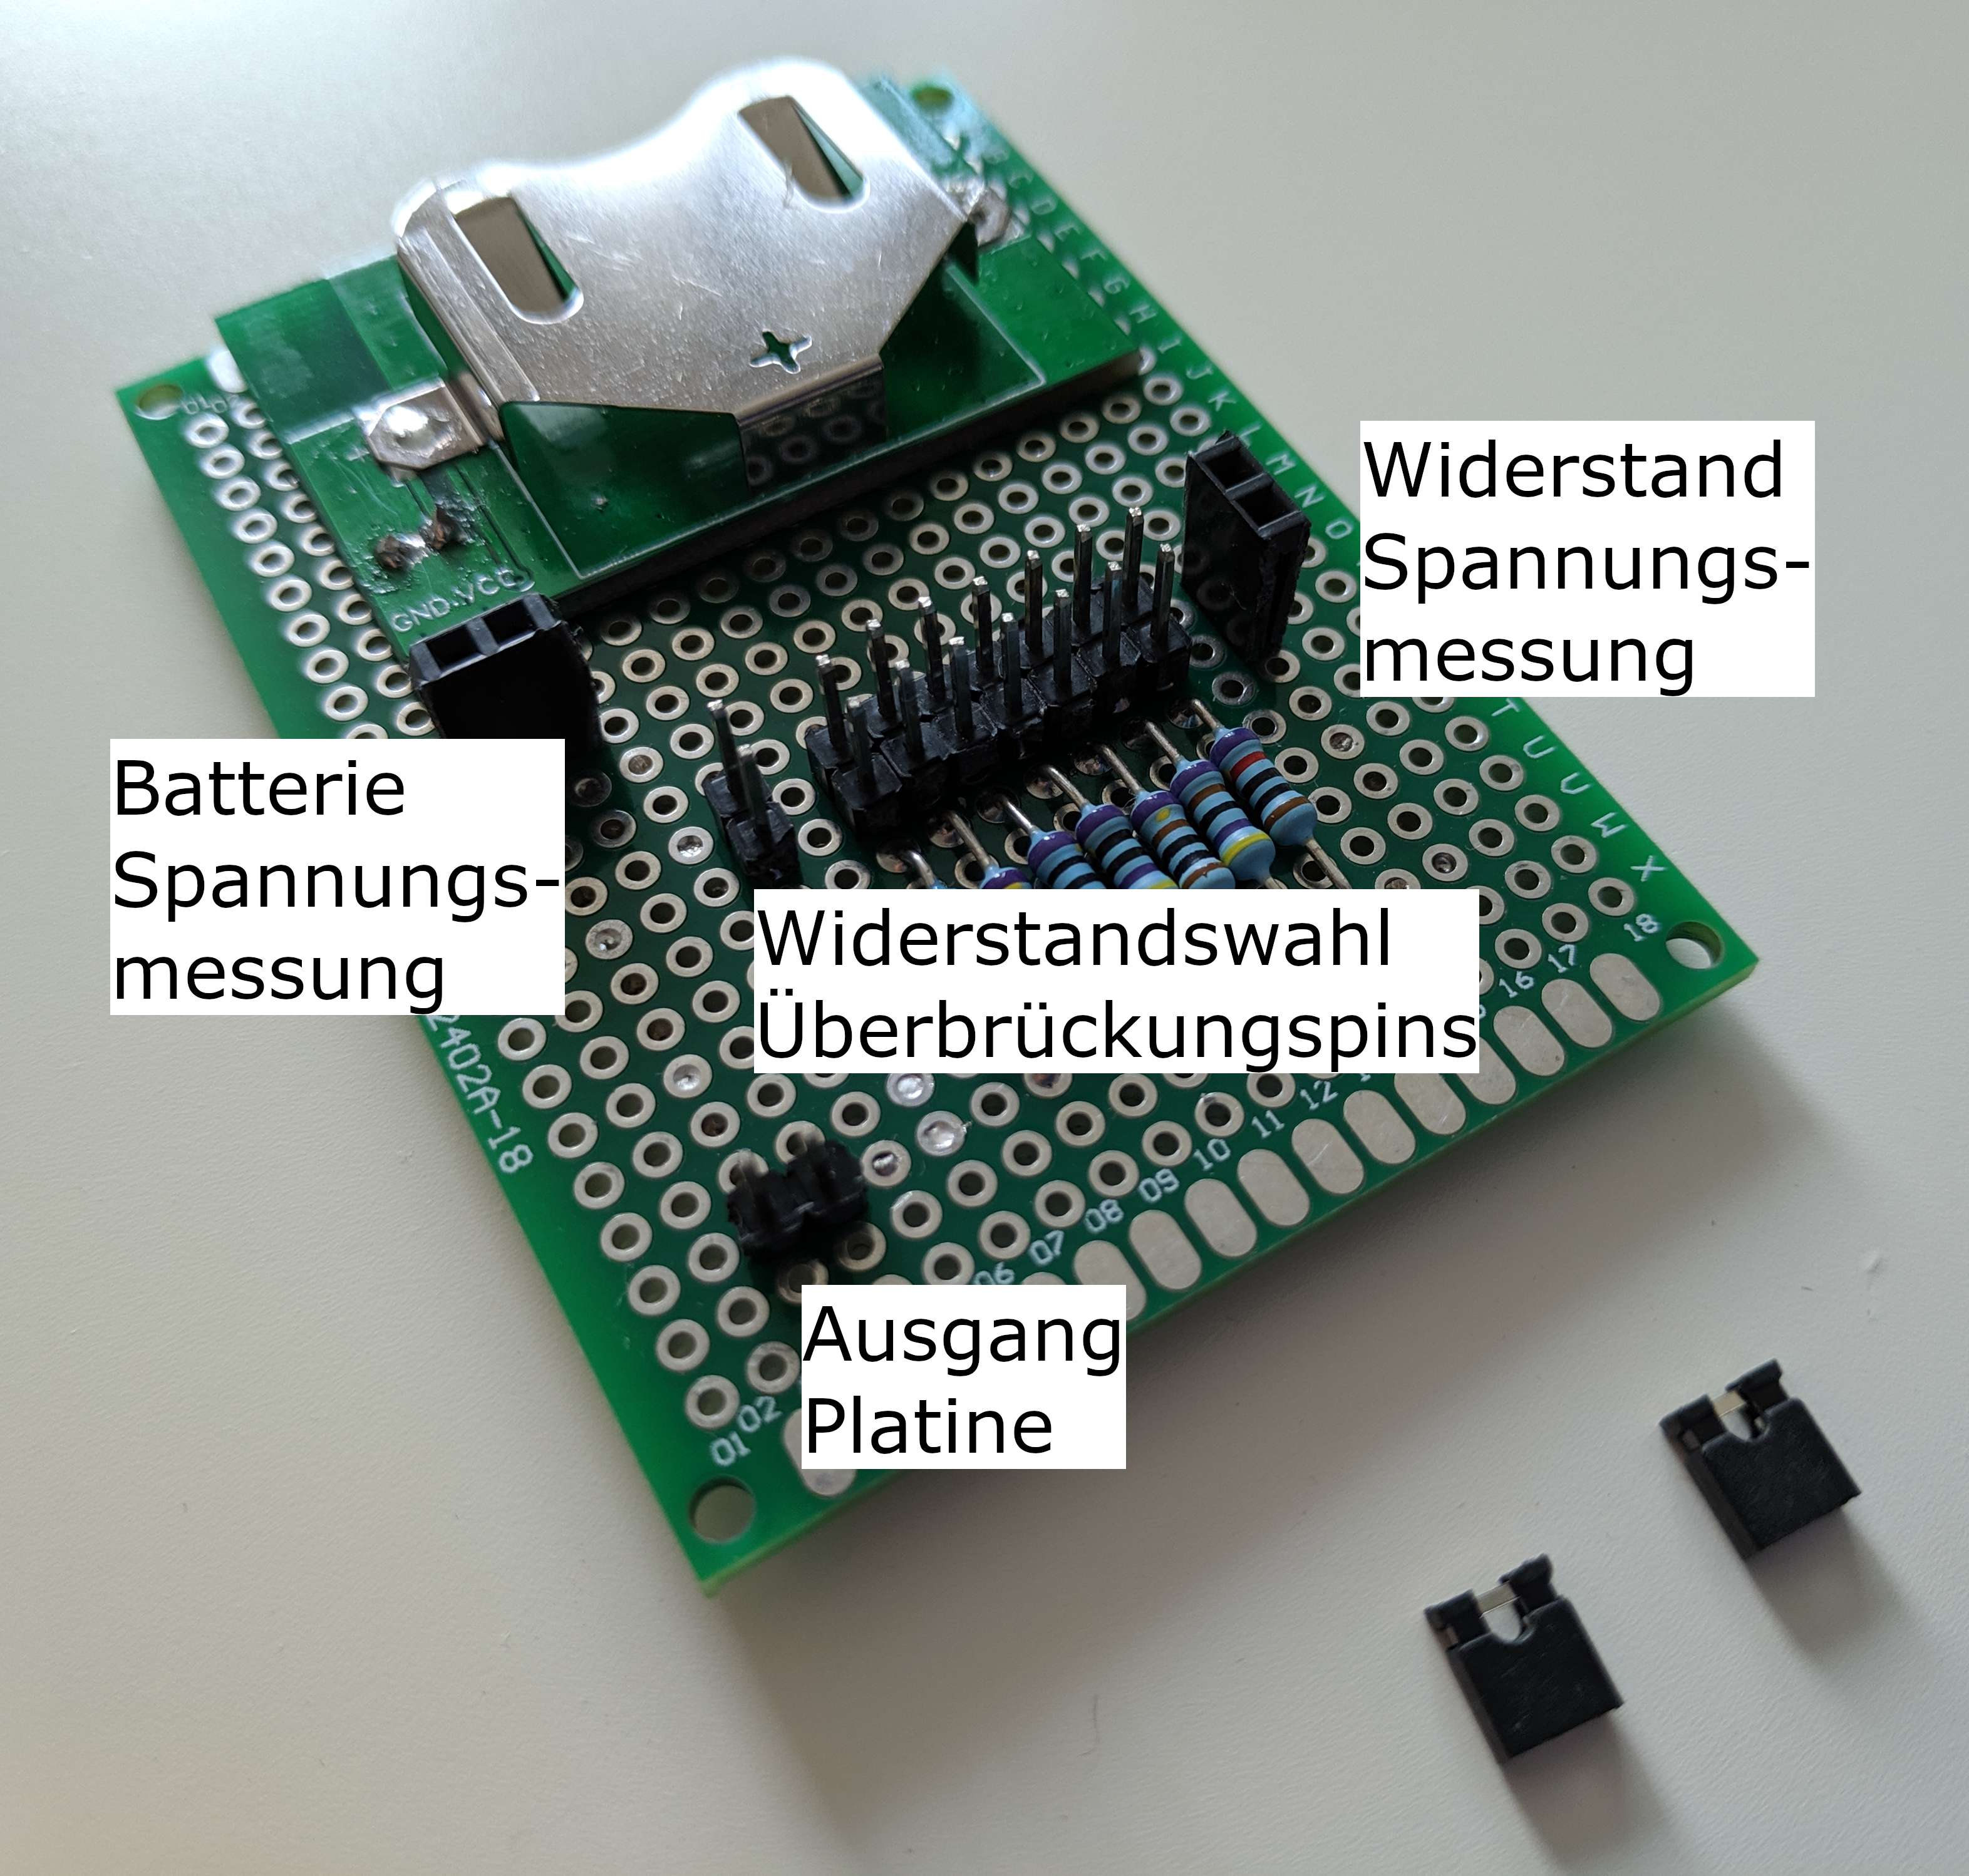
\includegraphics[width=0.45\linewidth]{res/messplatine.jpg}
	\caption{Messplatine}
	\label{fig:messplatine}
\end{figure}
Die Widerstände haben eine Toleranz von 0.1 \% und Werte von 0, 10, 47, 100, 470, 1000, 4700 und 10000 Ohm.\\
Das Oszilloskop ist ein Picoscope 5444B.
Der Spannungsabfall wird mit einer Frequenz von 2 GHz gemessen.
Technisch bedingt kann der Mittelwert nur über 5 Sekunden automatisch gebildet werden.
Deshalb wird jeder Test 6 Mal abgeschlossen, um Daten von 30 Sekunden zu erhalten.
Das Offset wird vor dem Test kalibriert.
Als Spannungsquelle wird eine neue CR2450 Knopfzelle und ein Voltcraft Model 2256 Netzgerät genutzt.
Da das Netzteil bei zu geringer Last keine stabile Spannung erzeugen kann, wird dem Testaufbau ein Widerstand von 58.75 Ohm +/- 5 \% parallel geschaltet.
Durch den Widerstand fließt dauerhaft etwa 51 mA, sodass das Netzteil mindestens eine Last von 3.4 \% hat.
Da das immer noch wenig ist, toleriert das Netzteil bei den Messungen einen geringeren Spannungsabfall bei den Messwiderständen als die Batterie.
Das Netzteil wird so eingestellt, dass am Testobjekt eine Spannung zwischen 2.95 und 3 V anliegt.
Es wird das Netzteil bei den Tests genutzt, bei denen der Prototyp involviert ist, da er sich zum Testzeitpunkt aus unbekannten Gründen nicht mit der Batterie starten lässt.
Zu einem späteren Zeitpunkt ist es hingegen wieder möglich.
Vor jeder Testreihe wird die Spannung am Netzteil nachjustiert oder die Spannung der Batterie notiert.\\
Beim Prototypen wird die Diode zum Verpolungsschutz mit SB12 überbrückt, wie in der Anleitung zum nRF52 DK angegeben \cite{site_nrf52dk}.
Der Spannungsabfall wird direkt an der Spannungsquelle gemessen und nicht an den Pins 'nRF current measurement'.
Nach dem Schaltbild von Figur 8 in \cite{site_nrf52dk} lässt sich sonst nur der Strom, der von der MCU aufgenommen wird, messen und der Verbrauch der IMU würde nicht mit eingehen.
Der Hinweis über Figur 8 besagt, dass die MCU bei der verwendeten Methode wegen der Reset-Funktion 20 $\mu$A mehr Strom verbraucht.
Da der Reset-Knopf erst eine Funktion zeigt, wenn auch SB10 überbrückt wird, kann keine Aussage getroffen werden, ob sich der Prototyp dahingehend vom Wearable unterschiedet.
Der Magnetometer wird beim BMI160 Shuttle Board wegen äußerer Umstände nicht entfernt oder konfiguriert.

\section{Ergebnisse}
Der erste Teil der Tabellen listet die Rahmenbedingungen für die Tests auf.
Die Zeilen der Daten beginnen mit der Beschreibung des Testfalls.
Die Zeile 'AVG' ist der Durchschnitt der sechs Einzeltests.
Sie besteht aus gemessenem Spannungsabfall und der berechneten Stromaufnahme.
Die Zeile 'P\textsubscript{AVG}' ist die Leistungsaufnahme nach $P_{AVG} = (Versorgungsspannung - gemesseneSpannung) * resultierender Strom$.
Die Versorgungsspannung wird beim Netzteil auf 2.975 V gemittelt.
Einzelne Tests haben zusätzlich die Standardabweichung 'ABW' oder listen die höchste gemessene Spitze im Spannungsabfall auf.

\begin{figure}[!hbtp]
  \begin{minipage}{0.5\textwidth}
    \centering
    \begin{tabular}{|l|l|l|}
      \hline
      Widerstand & \multicolumn{2}{l|}{10 Ohm}\\
      SPI-Frequenz & \multicolumn{2}{l|}{4 MHz}\\
      MTU-Größe & \multicolumn{2}{l|}{23 Byte}\\
      TX-Buffer & \multicolumn{2}{l|}{10 Einträge}\\
      Spannungsquelle & \multicolumn{2}{l|}{Netzteil}\\
      MCU & \multicolumn{2}{l|}{Wearable und Prototyp}\\
      IMU & \multicolumn{2}{l|}{LSM6DSL und BMI160}\\
      Sensordatenrate & \multicolumn{2}{l|}{200 Hz und 0 Hz}\\
      Connection Interval & \multicolumn{2}{l|}{High}\\
      \hline
      \multicolumn{3}{|c|}{Wearable LSM6DSL 200 Hz}\\
      AVG & 24.555 mV & 2.456 mA\\
      P\textsubscript{AVG} & \multicolumn{2}{c|}{7.246 mW}\\
      \hline
      \multicolumn{3}{|c|}{Wearable LSM6DSL 0 Hz}\\
      AVG & 3.55 mV & 355 $\mu$A\\
      P\textsubscript{AVG} & \multicolumn{2}{c|}{1.055 mW}\\
      \hline
      \multicolumn{3}{|c|}{Prototyp LSM6DSL 200 Hz}\\
      AVG & 29.455 mV & 2.946 mA\\
      P\textsubscript{AVG} & \multicolumn{2}{c|}{8.678 mW}\\
      \hline
      \multicolumn{3}{|c|}{Prototyp LSM6DSL 0 Hz}\\
      AVG & 10.153 mV & 1.015 mA\\
      P\textsubscript{AVG} & \multicolumn{2}{c|}{3.009 mW}\\
      \hline
      \multicolumn{3}{|c|}{Prototyp BMI160 200 Hz}\\
      AVG & 34.958 mV & 3.496 mA\\
      P\textsubscript{AVG} & \multicolumn{2}{c|}{10.278 mW}\\
      \hline
      \multicolumn{3}{|c|}{Prototyp BMI160 0 Hz}\\
      AVG & 10.031 mV & 1.003 mA\\
      P\textsubscript{AVG} & \multicolumn{2}{c|}{2.974 mW}\\
      \hline
    \end{tabular}
    \captionof{table}{Prototyp vs Wearable und BMI160 vs LSM6DSL}%
    \label{tab:test1}
  \end{minipage}
  \begin{minipage}{0.5\textwidth}
    \centering
    \begin{tabular}{|l|l|l|}
      \hline
      Widerstand & \multicolumn{2}{l|}{47 Ohm}\\
      SPI-Frequenz & \multicolumn{2}{l|}{1 MHz}\\
      MTU-Größe & \multicolumn{2}{l|}{23, 50 und 517 Byte}\\
      TX-Buffer & \multicolumn{2}{l|}{1, 50 und 300 Einträge}\\
      Algorithmus & \multicolumn{2}{l|}{An und Aus}\\
      Spannungsquelle & \multicolumn{2}{l|}{Batterie 3.044 V}\\
      MCU & \multicolumn{2}{l|}{Wearable}\\
      IMU & \multicolumn{2}{l|}{LSM6DSL}\\
      Sensordatenrate & \multicolumn{2}{l|}{200 Hz}\\
      Connection Interval & \multicolumn{2}{l|}{High}\\
      \hline
      \multicolumn{3}{|c|}{MTU23 TX1 Algo=An}\\
      AVG & 125.267 mV & 2.665 mA\\
      P\textsubscript{AVG} & \multicolumn{2}{c|}{7.778 mW}\\
      ABW & \multicolumn{2}{c|}{10.4 - 10.8 Hz}\\
      \hline
      \multicolumn{3}{|c|}{MTU23 TX50 Algo=An}\\
      AVG & 126.2 mV & 2.685 mA\\
      P\textsubscript{AVG} & \multicolumn{2}{c|}{7.834 mW}\\
      ABW & \multicolumn{2}{c|}{10.2 - 11.5 Hz}\\
      \hline
      \multicolumn{3}{|c|}{MTU23 TX300 Algo=An}\\
      AVG & 126.217 mV & 2.685 mA\\
      P\textsubscript{AVG} & \multicolumn{2}{c|}{7.836 mW}\\
      ABW & \multicolumn{2}{c|}{8.2 - 8.8 Hz}\\
      \hline
      \multicolumn{3}{|c|}{MTU23 TX1 Algo=Aus}\\
      AVG & 125.317 mV & 2.666 mA\\
      P\textsubscript{AVG} & \multicolumn{2}{c|}{7.781 mW}\\
      ABW & \multicolumn{2}{c|}{11.9 - 12.4 Hz}\\
      \hline
      \multicolumn{3}{|c|}{MTU23 TX50 Algo=Aus}\\
      AVG & 125.883 mV & 2.678 mA\\
      P\textsubscript{AVG} & \multicolumn{2}{c|}{7.815 mW}\\
      ABW & \multicolumn{2}{c|}{12 - 12.7 Hz}\\
      \hline
      \multicolumn{3}{|c|}{MTU23 TX300 Algo=Aus}\\
      AVG & 125.9 mV & 2.679 mA\\
      P\textsubscript{AVG} & \multicolumn{2}{c|}{7.818 mW}\\
      ABW & \multicolumn{2}{c|}{12 - 13.2 Hz}\\
      \hline
    \end{tabular}
    \captionof{table}{Größenänderung von TX-Buffer und MTU}%
    \label{tab:test2}
  \end{minipage}
\end{figure}

\begin{figure}[!hbtp]
  \begin{minipage}{0.5\textwidth}
    \centering
    \begin{tabular}{|l|l|l|}
      \hline
      \multicolumn{3}{|c|}{MTU150 TX10 Algo=An}\\
      AVG & 125.8 mV & 2.677 mA\\
      P\textsubscript{AVG} & \multicolumn{2}{c|}{7.812 mW}\\
      ABW & \multicolumn{2}{c|}{8.9 - 10.1 Hz}\\
      \hline
      \multicolumn{3}{|c|}{MTU517 TX10 Algo=An}\\
      AVG & 126.1 mV & 2.683 mA\\
      P\textsubscript{AVG} & \multicolumn{2}{c|}{7.829 mW}\\
      ABW & \multicolumn{2}{c|}{8.4 - 9.4 Hz}\\
      \hline
      \multicolumn{3}{|c|}{MTU150 TX50 Algo=An}\\
      AVG & 125.783 mV & 2.676 mA\\
      P\textsubscript{AVG} & \multicolumn{2}{c|}{7.809 mW}\\
      ABW & \multicolumn{2}{c|}{10.3 - 11.2 Hz}\\
      \hline
    \end{tabular}
    \captionof{table}{Fortsetzung von Tabelle \ref{tab:test2}}%
    \label{tab:test2b}
    \hfill \break
    \hfill \break
    \begin{tabular}{|l|l|l|}
      \hline
      Widerstand & \multicolumn{2}{l|}{47 Ohm}\\
      SPI-Frequenz & \multicolumn{2}{l|}{125 kHz, 1 MHz, 8 MHz}\\
      MTU-Größe & \multicolumn{2}{l|}{35 Byte}\\
      TX-Buffer & \multicolumn{2}{l|}{10 Einträge}\\
      Spannungsquelle & \multicolumn{2}{l|}{Batterie 3.044 V}\\
      MCU & \multicolumn{2}{l|}{Wearable}\\
      IMU & \multicolumn{2}{l|}{LSM6DSL}\\
      Sensordatenrate & \multicolumn{2}{l|}{400 Hz}\\
      Connection Interval & \multicolumn{2}{l|}{High}\\
      \hline
      \multicolumn{3}{|c|}{125kHz}\\
      AVG & 294.95 mV & 6.276 mA\\
      P\textsubscript{AVG} & \multicolumn{2}{c|}{17.253 mW}\\
      ABW & \multicolumn{2}{c|}{21.4 - 23 Hz}\\
      \hline
      \multicolumn{3}{|c|}{1MHz}\\
      AVG & 187.817 mV & 3.996 mA\\
      P\textsubscript{AVG} & \multicolumn{2}{c|}{11.413 mW}\\
      ABW & \multicolumn{2}{c|}{15.7 - 17.8 Hz}\\
      \hline
      \multicolumn{3}{|c|}{8MHz}\\
      AVG & 173.233 mV & 3.686 mA\\
      P\textsubscript{AVG} & \multicolumn{2}{c|}{10.582 mW}\\
      ABW & \multicolumn{2}{c|}{15.1 - 17.1 Hz}\\
      \hline
    \end{tabular}
    \captionof{table}{Frequenzänderung von SPI}%
    \label{tab:test3}
  \end{minipage}
  \begin{minipage}{0.5\textwidth}
    \centering
    \begin{tabular}{|l|l|l|}
      \hline
      Widerstand & \multicolumn{2}{l|}{47 Ohm}\\
      SPI-Frequenz & \multicolumn{2}{l|}{4 MHz}\\
      MTU-Größe & \multicolumn{2}{l|}{35 Byte}\\
      TX-Buffer & \multicolumn{2}{l|}{10 Einträge}\\
      Spannungsquelle & \multicolumn{2}{l|}{Batterie 2.991 V}\\
      MCU & \multicolumn{2}{l|}{Wearable}\\
      IMU & \multicolumn{2}{l|}{LSM6DSL}\\
      Sensordatenrate & \multicolumn{2}{l|}{0 und 100 Hz}\\
      Connection Interval & \multicolumn{2}{l|}{Low, Balance, High}\\
      \hline
      \multicolumn{3}{|c|}{Low 0Hz}\\
      AVG & 22.715 mV & 483.298 $\mu$A\\
      P\textsubscript{AVG} & \multicolumn{2}{c|}{1.434 mW}\\
      \hline
      \multicolumn{3}{|c|}{Balance 0Hz}\\
      AVG & 27.27 mV & 580.213 $\mu$A\\
      P\textsubscript{AVG} & \multicolumn{2}{c|}{1.719 mW}\\
      \hline
      \multicolumn{3}{|c|}{High 0Hz}\\
      AVG & 36.652 mV & 779.83 $\mu$A\\
      P\textsubscript{AVG} & \multicolumn{2}{c|}{2.304 mW}\\
      \hline
      \multicolumn{3}{|c|}{Low 100Hz}\\
      AVG & 83.443 mV & 1.775 mA\\
      P\textsubscript{AVG} & \multicolumn{2}{c|}{5.161
       mW}\\
       ABW & \multicolumn{2}{c|}{7.3 - 8.2 Hz}\\
      \hline
      \multicolumn{3}{|c|}{Balance 100Hz}\\
      AVG & 86.188 mV & 1.834 mA\\
      P\textsubscript{AVG} & \multicolumn{2}{c|}{5.327 mW}\\
      ABW & \multicolumn{2}{c|}{5.5 - 6.3 Hz}\\
      \hline
      \multicolumn{3}{|c|}{High 100Hz}\\
      AVG & 94.575 mV & 2.012 mA\\
      P\textsubscript{AVG} & \multicolumn{2}{c|}{5.828 mW}\\
      ABW & \multicolumn{2}{c|}{4.7 - 5.1 Hz}\\
      \hline
    \end{tabular}
    \captionof{table}{Änderung des Connection Intervals}%
    \label{tab:test4}
  \end{minipage}
\end{figure}

\begin{figure}[!hbtp]
  \begin{minipage}{0.5\textwidth}
    \centering
    \begin{tabular}{|l|l|l|}
      \hline
      Widerstand & \multicolumn{2}{l|}{47 Ohm}\\
      SPI-Frequenz & \multicolumn{2}{l|}{4 MHz}\\
      MTU-Größe & \multicolumn{2}{l|}{35 Byte}\\
      TX-Buffer & \multicolumn{2}{l|}{10 Einträge}\\
      Spannungsquelle & \multicolumn{2}{l|}{Batterie 2.991 V}\\
      MCU & \multicolumn{2}{l|}{Wearable}\\
      IMU & \multicolumn{2}{l|}{LSM6DSL}\\
      Sensordatenrate & \multicolumn{2}{l|}{25 bis 800 Hz}\\
      Connection Interval & \multicolumn{2}{l|}{High}\\
      \hline
      \multicolumn{3}{|c|}{25Hz}\\
      AVG & 78.043 mV & 1.66 mA\\
      P\textsubscript{AVG} & \multicolumn{2}{c|}{4.836 mW}\\
      \hline
      \multicolumn{3}{|c|}{50Hz}\\
      AVG & 83.378 mV & 1.774 mA\\
      P\textsubscript{AVG} & \multicolumn{2}{c|}{5.158 mW}\\
      \hline
      \multicolumn{3}{|c|}{100Hz}\\
      AVG & 98.362 mV & 2.093 mA\\
      P\textsubscript{AVG} & \multicolumn{2}{c|}{6.054 mW}\\
      \hline
      \multicolumn{3}{|c|}{200Hz}\\
      AVG & 125.233 mV & 2.665 mA\\
      P\textsubscript{AVG} & \multicolumn{2}{c|}{7.637 mW}\\
      \hline
      \multicolumn{3}{|c|}{400Hz}\\
      AVG & 180.817 mV & 3.847 mA\\
      P\textsubscript{AVG} & \multicolumn{2}{c|}{10.811 mW}\\
      \hline
      \multicolumn{3}{|c|}{800Hz}\\
      AVG & 286.167 mV & 6.089 mA\\
      P\textsubscript{AVG} & \multicolumn{2}{c|}{16.47 mW}\\
      \hline
    \end{tabular}
    \captionof{table}{Änderung der Sensordatenrate}%
    \label{tab:test5}
  \end{minipage}
  \begin{minipage}{0.5\textwidth}
    \centering
    \begin{tabular}{|l|l|l|}
      \hline
      Widerstand & \multicolumn{2}{l|}{47 und 10000 Ohm}\\
      SPI-Frequenz & \multicolumn{2}{l|}{8 MHz}\\
      MTU-Größe & \multicolumn{2}{l|}{23 Byte}\\
      TX-Buffer & \multicolumn{2}{l|}{17 Einträge}\\
      Spannungsquelle & \multicolumn{2}{l|}{Batterie 2.875 und 2.916 V}\\
      MCU & \multicolumn{2}{l|}{Wearable}\\
      IMU & \multicolumn{2}{l|}{LSM6DSL}\\
      \hline
      \multicolumn{3}{|c|}{PowerOff 10000Ohm 2.875V}\\
      Spitze & 61 mV & 6.1 $\mu$A\\
      AVG & 15.373 mV & 1.537 $\mu$A\\
      P\textsubscript{AVG} & \multicolumn{2}{c|}{0.006 mW}\\
      \hline
      \multicolumn{3}{|c|}{Advertising 47Ohm 2.916V}\\
      Spitze & 646 mV & 13.745 mA\\
      AVG & 35.787 mV & 761.426 $\mu$A\\
      P\textsubscript{AVG} & \multicolumn{2}{c|}{2.192 mW}\\
      \hline
    \end{tabular}
    \captionof{table}{Advertising und Schlafmodus}%
    \label{tab:test6}
  \end{minipage}
\end{figure}

\begin{figure}[!hbtp]
	\centering
	\includegraphics[width=1\linewidth]{res/idle.jpg}
	\caption{Wearable im Schlafmodus bei Batteriespannung}
	\label{fig:curSleep}
\end{figure}
\begin{figure}[!hbtp]
	\centering
	\includegraphics[width=1\linewidth]{res/wearNetzAdv.jpg}
	\caption{Advertising vom Wearable bei Netzteilspannung}
	\label{fig:curNetz}
\end{figure}
\begin{figure}[!hbtp]
	\centering
	\includegraphics[width=1\linewidth]{res/wearCrAdv.jpg}
	\caption{Advertising vom Wearable bei Batteriespannung}
	\label{fig:curCr}
\end{figure}
\begin{figure}[!hbtp]
	\centering
	\includegraphics[width=1\linewidth]{res/wearNetz0hz.jpg}
	\caption{Verbunden mit High CI und 0 Hz bei Netzteilspannung}
	\label{fig:curHiNetz}
\end{figure}
\begin{figure}[!hbtp]
	\centering
	\includegraphics[width=1\linewidth]{res/ciLo0.jpg}
	\caption{Verbunden mit Low CI und 0 Hz bei Batteriespannung}
	\label{fig:curLo}
\end{figure}
\begin{figure}[!hbtp]
	\centering
	\includegraphics[width=1\linewidth]{res/ciMi0.jpg}
	\caption{Verbunden mit Balance CI und 0 Hz bei Batteriespannung}
	\label{fig:curMi}
\end{figure}
\begin{figure}[!hbtp]
	\centering
	\includegraphics[width=1\linewidth]{res/ciHi0.jpg}
	\caption{Verbunden mit High CI und 0 Hz bei Batteriespannung}
	\label{fig:curHi}
\end{figure}
\begin{figure}[!hbtp]
	\centering
	\includegraphics[width=1\linewidth]{res/wearNetzteil200hz.jpg}
	\caption{Verbunden mit High CI und 200 Hz bei Netzteilspannung}
	\label{fig:cur200}
\end{figure}

\section{Auswertung}
Zunächst ist zu beachten, dass der Ausschlag der Spannungen in den Abbildungen \ref{fig:curSleep} bis \ref{fig:cur200} teilweise negativ ist.
Es hat keinerlei Auswirkungen auf die Daten und ist durch die Messweise bedingt.
Ein Abschnitt auf der X-Achse sind 0.5 Sekunden, sodass eine komplette Abbildung 5 Sekunden darstellt.
Eine Frequenz von 0 Hz bedeutet, dass die IMU keine Daten erfasst.

\subsection{Strommessung mithilfe eines Widerstandes}
Vergleicht man Abbildung \ref{fig:curNetz} und Abbildung \ref{fig:curCr}, stellt man fest, dass sich die Verlaufskurven bei Batterie- und Netzspannung nicht unterscheiden.
Es sind regelmäßige Spitzen zu erkennen in denen das Wearable am Advertisen ist.
Die zusätzliche Stromaufnahme durch die blinkende LED ist beobachtbar.\\
Vergleicht man den Strom in 'Wearable LSM6DSL 200 Hz' (Tabelle \ref{tab:test1}) mit dem von '200Hz' (Tabelle \ref{tab:test5}), stellt man einen Anstieg der Stromaufnahme von 8.51 \% bei Batteriebetrieb fest.
Werden die Werte 'Wearable LSM6DSL 0 Hz' (Tabelle \ref{tab:test1}) und 'High 0Hz' (Tabelle \ref{tab:test4}) verglichen, sind die Unterschiede noch höher.
Beim Batteriebetrieb hier ist die Stromaufnahme 120 \% höher.
Es war nicht zu erwarten, dass eine Änderung der Spannungsquelle derartigen Unterschied verursacht.
Es handelt sich nicht wie zunächst angenommen um eine falsche Einstellung des Wearables.
Abbildung \ref{fig:curHiNetz} zeigt die zugehörige Aufnahme, die dem Muster von Abbildung \ref{fig:curHi} entspricht.\\
In Tabelle \ref{tab:test1} wurde mit einem 10 Ohm Widerstand gemessen, wohingegen in Tabelle \ref{tab:test5} mit 47 Ohm gemessen wurde.
Während die Spannungsquellen beide etwa 3 Volt liefern, fällt eine unterschiedliche Spannung an den Widerständen ab.
In den Datenblättern der Komponenten ist die Stromaufnahme bei einer bestimmten Spannung spezifiziert \cite{datasheet_lsm6dsl} \cite{datasheet_nrf52832}.
Bei der eingesetzten Messmethode ist die Spannung am Testobjekt abhängig von dem Spannungsabfall über die Widerstände, der von der Stromaufnahme des Wearables bestimmt wird.\\
Unter der Annahme, dass das Wearable die geringere Spannung mit einem höheren Strom ausgleicht, wurde die Berechnung der Leistungsaufnahme zu den Daten hinzugefügt.
Auch hier lässt bei den vorherigen Szenarien ein Anstieg der Leistungsaufnahme bei Batteriebetrieb von 5.4 \% bzw. 118 \% verzeichnen.\\
Eine weitere Fehleranalyse hat ergeben, dass die Abweichung der Messwerte durch die Erhöhung des Widerstandes zustande kommen muss.
So bedeutet ein höherer Messwiderstand auch einen höheren Leistungsverlust durch den Widerstand.
Statt den Widerstand zu erhöhen, wird normalerweise der geringe Spannungsabfall mit einem analogen Frontend (AFE) erhöht. \cite{site_strommessung}\\
Der Messwiderstandwert von 10 Ohm ist für die MCU alleine empfohlen.
Von der Testreihe sind damit nur die Messwerte 'Prototyp BMI160 0 Hz', 'Prototyp LSM6DSL 0 Hz' und 'Wearable LSM6DSL 0 Hz' von Tabelle \ref{tab:test1} korrekt, da die IMU in den Testfällen ausgeschaltet war und mit einem 10 Ohm Widerstand gemessen wurde.
Die anderen Messungen können bei einem Vergleich untereinander einen Einblick gewähren, welche Szenarien eine höhere Stromaufnahme verursachen, solange die Widerstände identisch sind.
Eine höhere Stromaufnahme bedeutet dabei einen höheren Leistungsverlust am Messwiderstand.
Die genauen Werte sind dabei nicht aussagekräftig.

\subsection{Stromeinfluss der Parameter}
Den wertkorrekten Testfällen kann man entnehmen, dass der Stromverbrauch des Prototypen das 2.86-fache des Stromverbrauches des Wearables beträgt.
Der BMI160 hat einen um 12 $\mu$A geringeren Stromverbrauch als der LSM6DSL, obwohl die Platine des BMI160 zusätzlich den Magnetometer beinhaltete.\\\\
Werden die IMUs bei 200 Hz betrieben, hat der BMI160 einen höheren Messwert als der LSM6DSL verzeichnet.
Bei 200 Hz verbraucht das Wearable weniger Strom als der Prototyp.\\
Betrachtet man Tabelle \ref{tab:test2}, so stellt man fest, dass die Größe des TX-Buffers und die Größe der MTU in der Stromaufnahme keinen einen Unterschied ausmachen, da sich hier alle Werte um maximal 0.78 \% voneinander unterscheiden.\\
Tabelle \ref{tab:test3} zeigt, dass die kleinstmögliche SPI-Frequenz mehr Leistung als die Höchstmögliche verbraucht.
Die mittlere Frequenz befindet sich dazwischen.
Das ist damit zu begründen, dass die Chipkommunikation schneller abgearbeitet und damit länger im Schlafmodus verblieben werden kann.\\
Tabelle \ref{tab:test4} sagt aus, dass eine Erhöhung des Connection Intervals die Stromaufnahme steigert.
Das ist zu erwarten, da die MCU öfter Daten ans Smartphone überträgt.
In den Abbildungen \ref{fig:curLo} bis \ref{fig:curHi} sieht man die Erhöhung der Anzahl der Spitzen proportional zum Connection Interval.\\
Tabelle \ref{tab:test5} zeigt, dass eine höhere Sensordatenrate auch eine höhere Stromaufnahme bedeutet.
Zum Einen wird die IMU stärker beansprucht und die FIFO muss öfter geleert werden.
Zum Anderen werden mehr Daten ans Smartphone verschickt.
Die Sensordatenrate von 800 Hz mit 4 MHz SPI-Frequenz hat dabei weniger Strom verbraucht als eine Sensordatenrate von 400 mit 125 kHz SPI-Frequenz\\
Abbildung \ref{fig:curSleep} zeigt die Stromaufnahme während des Schlafmodus der MCU.
Es sind regelmäßig Stromspitzen zu sehen.
Sie kommen daher, dass die MCU einen internen Spannungswandler besitzt.
Wenn der benötigte Strom gering ist, wird der Spannungswandler in Intervallen betrieben und lädt dabei einen Kondensator auf, von dem die MCU ihre Leistung beziehen kann \cite{site_refreshMode}.\\\\
Anhand der Daten ist davon auszugehen, dass die Stromaufnahme in der tatsächlichen Nutzung über 1 mA beträgt.
Das entspricht 2 - 3 kOhm bei 2 - 3 V.
Während die CR2450 bei 3 kOhm weniger als 90 \% der Kapazität besitzt und für 2 kOhm nicht mehr spezifiziert ist \cite{datasheet_ds6450}, behält die CR2032 bei dem Widerstand noch etwa die gesamte Kapazität \cite{datasheet_ds6032}.
Bei 550 mAh soll sich die CR2450 bei 1 mA und 3 kOhm etwa 23 Tage betreiben lassen.\\
Um höhere Stromaufnahmen zu unterstützen, wurde nach einem anderen Batteriemodell gesucht, das sich für hohe Ströme eignet.
Die Murata CR2450R werden explizit als ``High Drain lithium coin batteries'' \cite{site_murataCr2450r} vermarktet.
Sie haben nur eine Kapazität von 500 mAh aber die Kapazität ist bis 10 mA angegeben und der Spitzenstrom darf 50 mA betragen.
Es wird empfohlen sie unter 3 mA zu betreiben, wo sie noch etwa 450 mAh bereitstellen kann.
Das ergibt eine Laufzeit von mehr als 6 Tagen bei 3 mA. \cite{site_murataCr2450r}\\
Wird die Hochstrom-CR2450 mit der CR2032 der selben Modellreihe verglichen, hat die CR2450 bei 3 mA die 2.5-fache Kapazität \cite{site_murataCr2032r}.
Dagegen hat der vorherige Vergleich in Abschnitt \ref{ch:aimEval} die 2.7-fache Kapazität ergeben.
Das Volumen beträgt weiterhin das 2.34-fache bei der CR2450.

\subsection{Standardabweichung der ankommenden Datenrate}
Bei allen Einstellungen ist die in der IMU eingestellte Datenrate beim Smartphone angekommen.
Die Standardabweichung hat sich allerdings bei den Einstellungen unterschieden.
Für die Standardabweichung ist ein Intervall angegeben, da die ausgegebenen Werte um etwa 0.5 Hz schwanken.
Dementsprechend muss eine hohe Ungenauigkeit berücksichtigt werden.\\
In Tabelle \ref{tab:test2} ist die Standardabweichung um mindestens 1 Hz höher wenn der Algorithmus nicht genutzt wird.
Damit kann ein positiver Effekt des Algorithmus auf die Abweichung der Datenrate beobachtet werden.\\
Die größte Einstellung des TX-Buffers bei aktiviertem Algorithmus hat eine etwa 2 Hz geringe Standardabweichung.
Die mittlere Einstellung des TX-Buffers hat in den Tests 'MTU23 TX50 Algo=An', 'MTU23 TX50 Algo=Aus' und 'MTU150 TX50 Algo=An' jeweils schlechtere Abweichungen als die zugehörige kleinste Einstellung ergeben.
Eine Vergrößerung der MTU hat die Standardabweichung verbessert.
Das war nicht zu Erwarten gewesen, da das übertragene Paket, die Struktur \texttt{imu\_data\_t}, eine Größe von 16 Byte besitzt und damit eine größere MTU nicht nötig schient.\\
Tabelle \ref{tab:test3} zeigt eine 4 Hz höhere Standardabweichung bei 125 kHz SPI-Frequenz, gegenüber höheren Frequenzen.
Das kann daher resultieren, dass die Übertragung der Daten von der FIFO so langsam abläuft, dass sie erst zum nächsten Connection Interval abgeschlossen wird.\\
Tabelle \ref{tab:test4} zeigt, dass sich die Standardabweichung mit zunehmendem Connection Interval um bis zu 3 Hz verbessert.
Wenn die Sensordaten in wenigen großen Burst übertragen werden, ist es wahrscheinlicher, dass ein Datum erst in der nächsten Sekunde ankommt.
Dadurch erhöht sich die Abweichung von der Sensordatenrate am Smartphone.
